\section{Explained through Baseball}

\begin{frame}
 \frametitle{Replica di dati nel cloud}
 \begin{itemize}
   \item Sistemi di cloud storage replicano i dati su più macchine per la tolleranza ai guasti e per beneficiare delle prestazioni.
   \item Sempre più spesso utilizzano la geo-replication per sopravvivere ad una eventuale perdita di datacenter.
   \item I datacenter vengono distribuita a livello globale in più continenti per garantire che i dati siano vicini a una base di client.
 \end{itemize}
  
\end{frame}

\begin{frame}
 \frametitle{Sistemi di storage popolari}
Attualmente i cloud storage systems offrono principalmente la strong consistency e eventual consistency:
 \begin{itemize}
   \item Amazon S3 – eventual consistency
   \item Amazon Simple DB – eventual o strong
   \item Google App Engine – strong o eventual
   \item Yahoo! PNUTS – eventual o strong
   \item Windows Azure Storage – strong o eventual
   \item Cassandra – eventual o strong
 \end{itemize}
%Amazon ha spinto sulla eventual consistency, ma le offerte sono per la strong consistency, un opzione aggiuntiva per servizi, come SimpleDB e DynamoDB.
%Google App Engine ha cominciato offrendo solo strong consistency, ma dopo ha aggiunto delle opzioni di lettura, weakly consistent data per quelle applicazioni che richiedono maggiori performance.
%Yahoo!’s PNUTS system, la tencologia di base per molti dei servizi offerti da Yahoo, offre sia eventual consistency e strong consistency.
%Windows Azure fornisce solo la strong consistency, anche se utilizza l'eventual consistency per i dati geo-replicati.
\end{frame}

\begin{frame}
\frametitle{Teorema CAP (Teorema di Bremer)}
	\begin{definizione}
	 Il \alert{teorema CAP} afferma che è impossibile per un sistema informatico distribuito fornire simultaneamente tutte e tre le seguenti garanzie:
	\begin{itemize}
		\item Coerenza\\
		tutti i nodi vedono gli stessi dati nello stesso momento
		\item Disponibilità\\
	    la garanzia che ogni richiesta riceva una risposta su ciò che sia riuscito o fallito
		\item Tolleranza di partizione\\
		il sistema continua a funzionare nonostante arbitrarie perdite di messaggi
	\end{itemize}
	Secondo il teorema, un sistema distribuito è in grado di soddisfare al massimo due di queste garanzie allo stesso tempo, ma non tutte e tre
	\end{definizione}
\end{frame}

\begin{frame}
\frametitle{Alcuni tipi di consistenza}
\begin{enumerate}
  \item \textbf{Strong Consistency}: garantisce che l'operazione di lettura ritorni il valore dell'ultima scrittura.
  \item \textbf{Eventual Consistency}: è la più debole delle altre, poiché permette di avere come valore di ritorno il più grande insieme di possibilità.
  \item \textbf{Consistent Prefix}: osserva l'ordine di sequenza delle scritture e ritorna l'ultima.
  \item \textbf{Bounded Staleness}: assicura che il risultato della lettura non sia scaduto, ovvero per ogni dato definisce un periodo di tempo $T$ 'staleness' e garantisce che l'operazione di lettura ritorni un qualsiasi valore scritto fra $T$ e il più recente.
  \item \textbf{Monotonic Reads}: si possono leggere dati stantii, ovvero se il client effettua la lettura di un dato ed ottiene un certo valore $X$ è garantito che se rilegge non riceverà un dato che è stato scritto prima di $X$. 
  \item \textbf{Read My Writes}: gli effetti di tutte le scritture che sono state fatte da un client, sono visibili al client successivo che legge quei dati.
\end{enumerate}
\end{frame}

\begin{frame}
\frametitle{Consistenze a confronto}
	\begin{figure}
		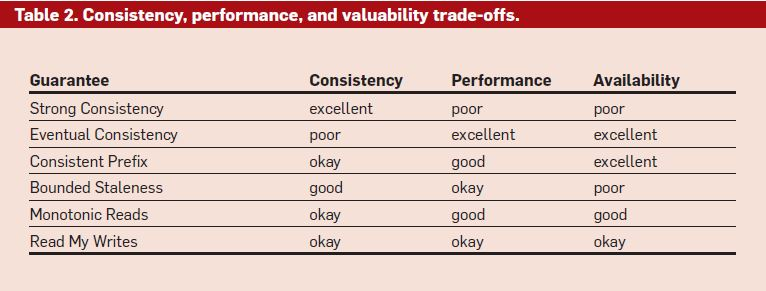
\includegraphics[scale=0.5]{baseball/tab2.jpg}
	\end{figure}
\end{frame}

\begin{frame}[fragile]
\frametitle{Il baseball in pseudocodice}
\begin{verbatim}
 Write ("visitors", 0);
 Write ("home", 0);
   for inning = 1 .. 9
     outs = 0;
     while outs < 3
       visiting player bats;
       for each run scored
         score = Read ("visitors");
         Write ("visitors", score + 1);
     outs = 0;
     while outs < 3
       home player bats;
       for each run scored
         score = Read ("home");
         Write ("home", score + 1);
 end game;
\end{verbatim}
\end{frame}

\begin{frame}
\frametitle{Un esempio}
	\begin{figure}
		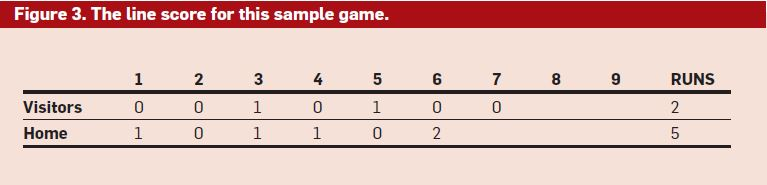
\includegraphics[scale=0.4]{baseball/tab3a.jpg}\\
		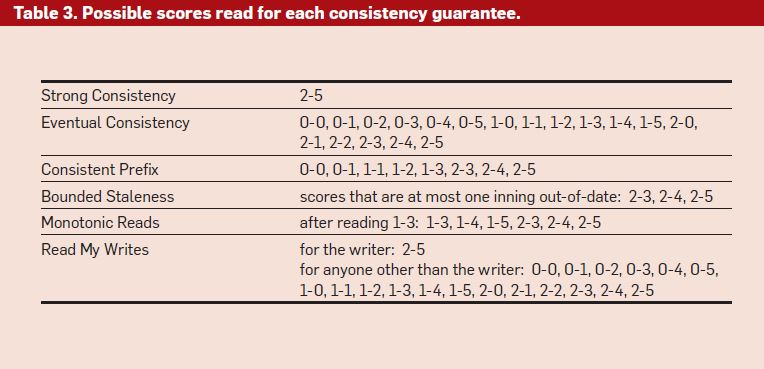
\includegraphics[scale=0.4]{baseball/tab3.jpg}
	\end{figure}
\end{frame}
